\documentclass{article}
\newenvironment{standalone}{\begin{preview}}{\end{preview}}
\usepackage{../includes}
\externaldocument{introduccion}
\externaldocument{modelo}

\begin{document}
\begin{standalone}
  \section{Resultados}

  \subsection{Observaciones en el osciloscopio}

  Conectamos las salidas de los canales analógicos a un osciloscopio MSO 2024B de la marca Tektronix.
  Este osciloscopio, que puede apreciarse en la \cref{fig:osciloscopio}, posee cuatro entradas analógicas y acepta señales de hasta 200 MHz, por lo que es ideal para nuestra aplicación.

  \begin{figure}[!htbp]
    \centering
    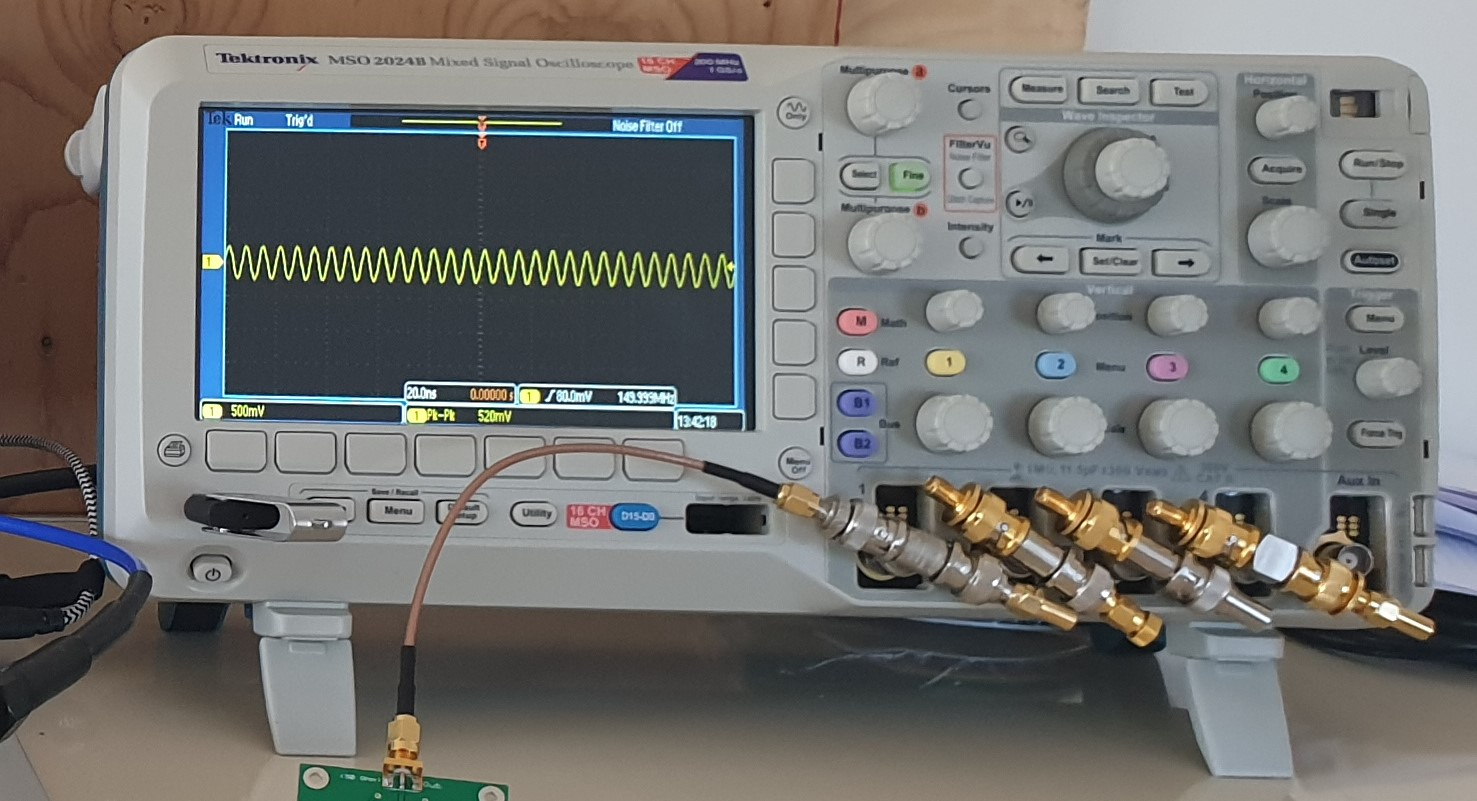
\includegraphics[width=\linewidth, height=50mm, keepaspectratio]{../images/osciloscopio.jpg}
    \caption{Osciloscopio Tektronix MSO 2024B.}
    \label{fig:osciloscopio}
  \end{figure}

  Capturamos nueve momentos de la pasada del sátelite a intervalos regulares y obtuvimos las imágenes que se pueden observar en la \cref{fig:pasada-osciloscopio}.

  \begin{figure}[!htbp]
    \centering

    \begin{tabular}{lccccc}
      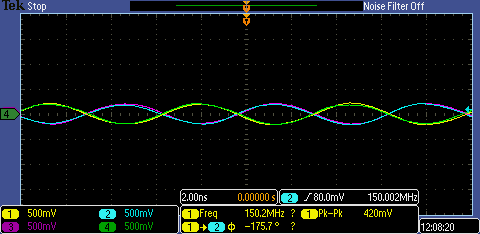
\includegraphics[width=\linewidth/3]{../images/pasada-osciloscopio/pasada1.png}&
      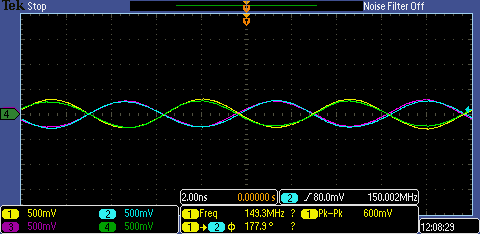
\includegraphics[width=\linewidth/3]{../images/pasada-osciloscopio/pasada2.png}&
      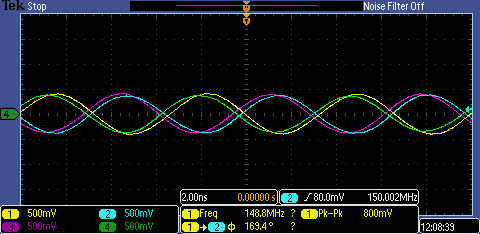
\includegraphics[width=\linewidth/3]{../images/pasada-osciloscopio/pasada3.png}\\
      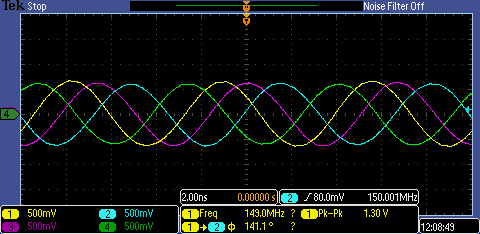
\includegraphics[width=\linewidth/3]{../images/pasada-osciloscopio/pasada4.png}&
      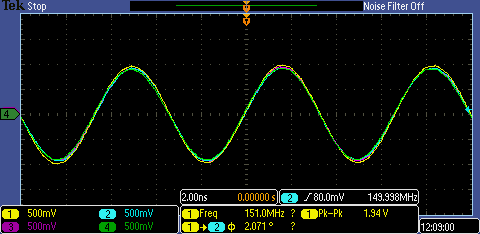
\includegraphics[width=\linewidth/3]{../images/pasada-osciloscopio/pasada5.png}&
      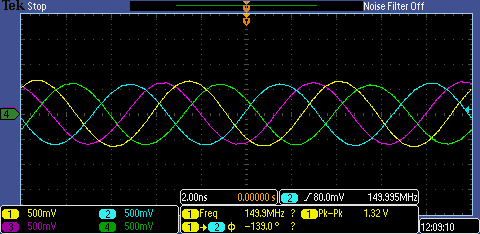
\includegraphics[width=\linewidth/3]{../images/pasada-osciloscopio/pasada6.png}\\
      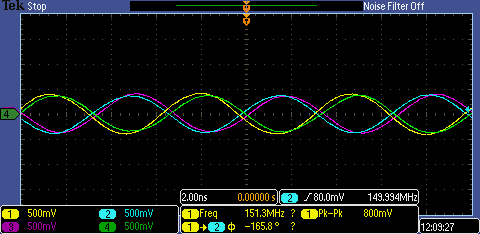
\includegraphics[width=\linewidth/3]{../images/pasada-osciloscopio/pasada7.png}&
      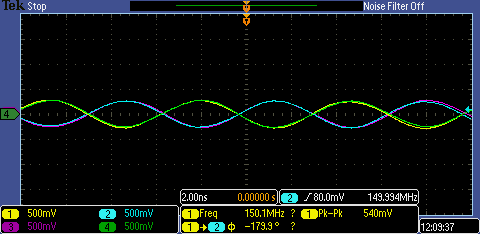
\includegraphics[width=\linewidth/3]{../images/pasada-osciloscopio/pasada8.png}&
      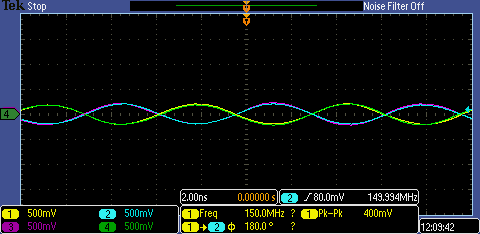
\includegraphics[width=\linewidth/3]{../images/pasada-osciloscopio/pasada9.png}\\
    \end{tabular}

    \caption{Capturas del osciloscopio para una pasada del satélite}
    \label{fig:pasada-osciloscopio}
  \end{figure}

  Podemos constatar que tanto la amplitud como la fase de las señales se corresponden con lo que esperábamos.
  Cuando el satélite aparece por el horizonte, la amplitud es mínima y las señales de elementos consecutivos están en contrafase.
  A medida que el satélite avanza, la amplitud y el desfase de las señales aumenta.
  Al llegar al cénit, la amplitud es máxima y todas las señales están en fase.
  El proceso inverso ocurre a partir de que el sátelite pasa por el cénit hasta que se oculta en el otro horizonte.

  Sin embargo, no es posible ver el corrimiento de frecuencia de las señales porque, para la frecuencia base analizada, 150 MHz, las variaciones de frecuencia presentes ($\pm$ 4 kHz) son menores a la resolución del osciloscopio.
  Por ello, recurrimos a un analizador de espectro para poder observar con precisión la frecuencia de las señales.

  \subsection{Observaciones en el analizador de espectro}

  Utilizamos un analizador de espectro N9320B de la empresa Keysight.
  Este equipo, ver \cref{fig:analizador-espectro}, trabaja con frecuencias de 9 kHz a 3 GHz.

  \begin{figure}[!htbp]
    \centering
    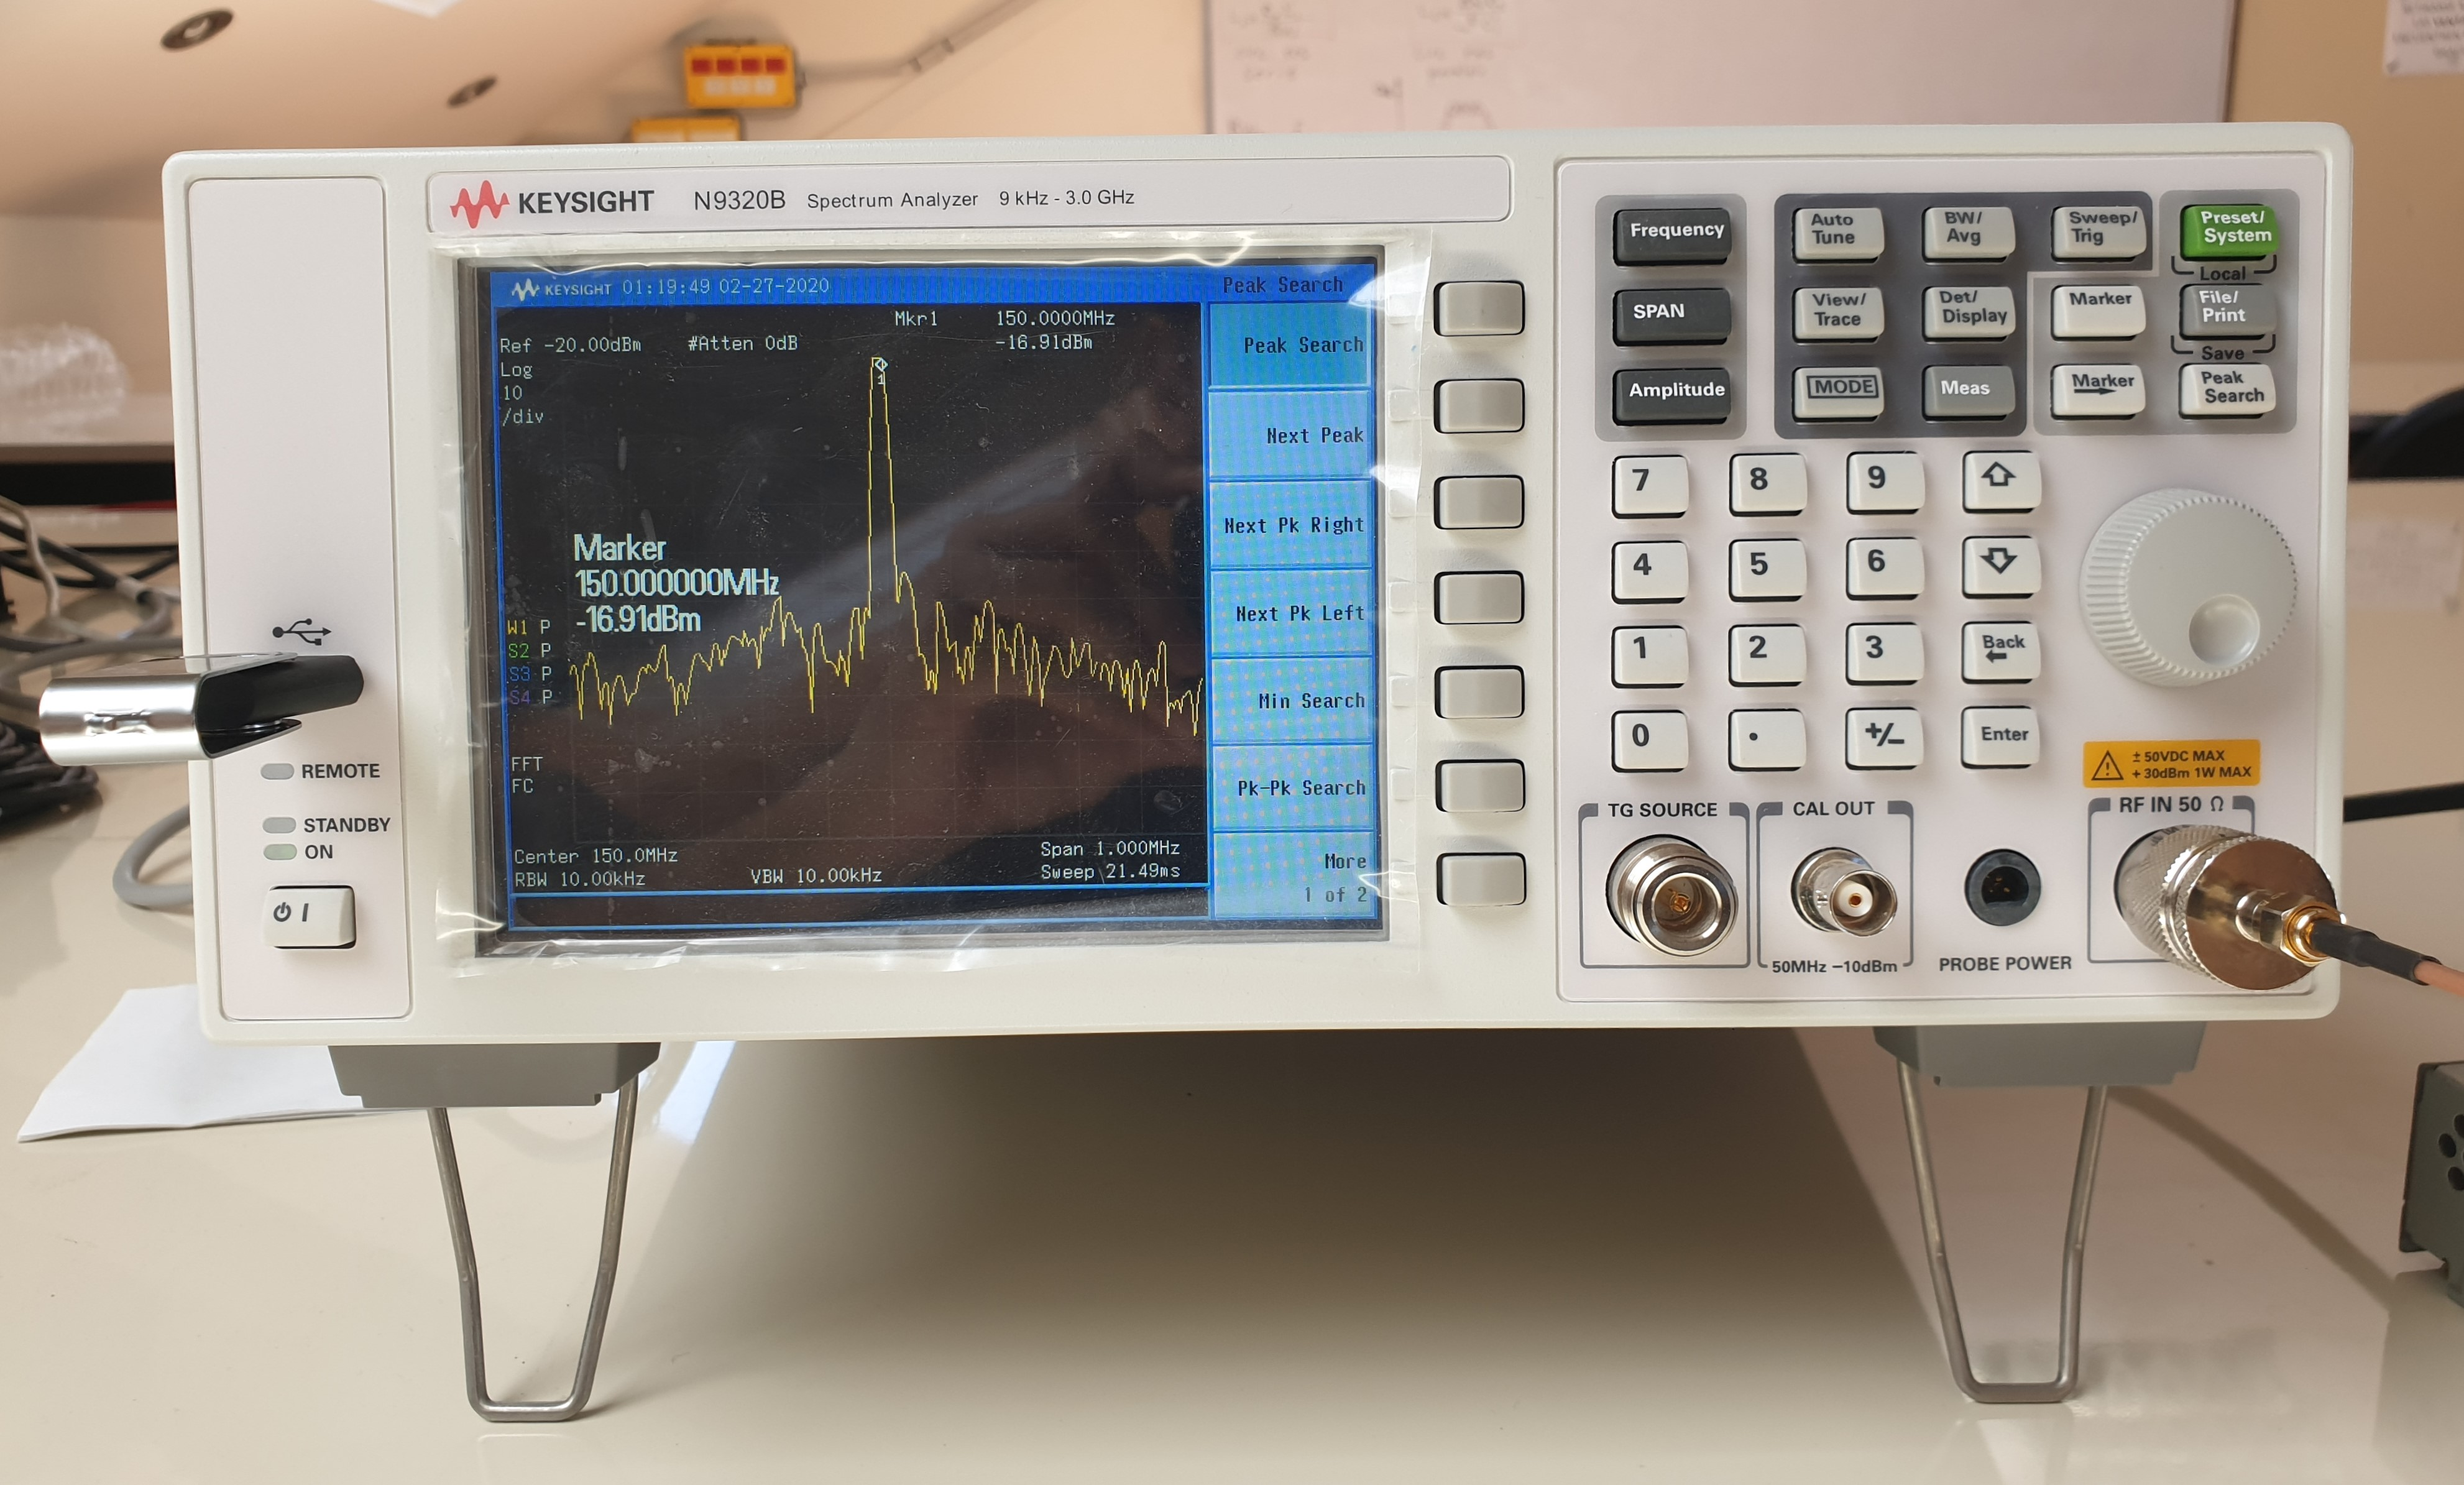
\includegraphics[width=\linewidth, height=50mm, keepaspectratio]{../images/analizador-espectro.jpg}
    \caption{Analizador de espectro Keysight N9320B.}
    \label{fig:analizador-espectro}
  \end{figure}

  Ya que la frecuencia es la misma para las cuatro señales, conectamos una sola salida del sintetizador al analizador de espectro.
  Con la función \textit{max-hold}, que mantiene los valores máximos en el tiempo, analizamos los mismos nueve momentos de la pasada del satélite y obtuvimos los resultados de la \cref{fig:pasada-analizador-espectro}.

  \begin{figure}[!htbp]
    \centering
    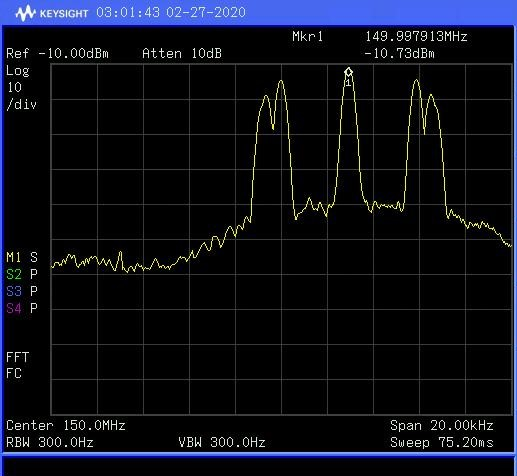
\includegraphics[width=\linewidth, height=80mm, keepaspectratio]{../images/pasada-analizador-espectro.jpg}
    \caption{Captura \textit{max-hold} del analizador de espectro para una pasada del satelite.}
    \label{fig:pasada-analizador-espectro}
  \end{figure}

  Podemos ver que existe un corrimiento en la frecuencia a lo largo del tiempo.
  Los picos pequeños al extremo derecho e izquierdo corresponden, respectivamente, al inicio y fin de la pasada.
  El pico máximo en el medio corresponde al momento en que el satélite está en el cénit del arreglo.
  Esto se corresponde con lo estudiado en el \cref{sec:modelo-senales}.
  Cuando el satélite aparece por un horizonte, éste se aproxima a la estación terrena y la frecuencia observada es máxima, cuando se esconde por el otro horizonte, se aleja y la frecuencia observada es mínima.

  Podemos observar que la frecuencia central no se encuentra exactamente en 150 MHz.
  Esto se debe a imprecisiones en el cristal del sintetizador digital directo.
  No obstante, el corrimiento sí se corresponde a lo calculado, 4 kHz.

  Analizamos además la respuesta en frecuencia del sintetizador digital directo para entender mejor su funcionamiento.
  Producimos una salida sinusoidal de 150 MHz y vemos en la \cref{fig:espurios} cómo aparecen espurios debidos a mezclas y alinealidades de los componentes.

  \begin{figure}[!htbp]
    \centering
    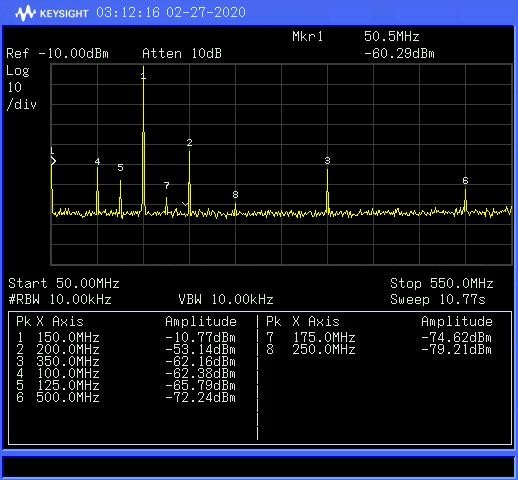
\includegraphics[width=\linewidth, height=80mm, keepaspectratio]{../images/espurios.jpg}
    \caption{Frecuencias espurias debido a mezclas y alinealidades de los componentes del sintetizador.}
    \label{fig:espurios}
  \end{figure}

  Por la teoría del muestreo, se explica que aparezca una imagen de la frecuencia de salida en
  \begin{equation}
    F_s - F_{out} = 500 \ \si{\mega\hertz} - 150 \ \si{\mega\hertz} = 350 \ \si{\mega\hertz}. \nonumber
  \end{equation}
  Por este motivo, los digitalizadores digitales directos incorporan un filtro pasa-bajo para mitigar este efecto.
  Producimos con el DDS un barrido de frecuencia de igual amplitud y observamos cómo es la respuesta del filtro en la \cref{fig:filtro-dds}

  \begin{figure}[!htbp]
    \centering
    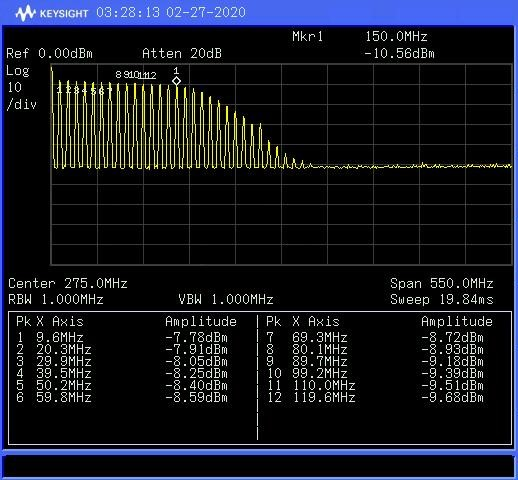
\includegraphics[width=\linewidth, height=80mm, keepaspectratio]{../images/filtro-dds.jpg}
    \caption{Respuesta en frecuencia del filtro pasa-bajo que incorpora el sintetizador.}
    \label{fig:filtro-dds}
  \end{figure}

  \subsection{Validación experimental del apuntamiento de haz}

  Vimos en el \cref{subsec:arreglo} que al sumar las señales de los elementos del arreglo, debido a interferencia constructiva y destructiva, se produce un apuntamiento de haz, es decir, existe una dirección en la cual la señal recibida es máxima.
  Si no hay ningún retardo entre las señales recibidas, el apuntamiento será hacia el cénit.
  Cuando introducimos un retardo entre las señales, el apuntamiento cambiará.

  Para validar este fenómeno, sumamos las señales de salida del sintetizador usando, en primer lugar, cables de igual longitud.
  Los cables de igual longitud producen retardos iguales en las señales.
  Obsarvamos la suma de las señales en el osciloscopio para una pasada del satélite y pudimos corroborar que la máxima señal se daba en $\theta = 0\degree$.


  Si tenemos cables de diferentes longitudes, el retardo entre las señales $t_{\text{offset}}$ esperado es
  \begin{equation}
    t_{\text{offset}} = \frac{\Delta l}{v},
    \tagaddtext{[\si{\second}]}
  \end{equation}
  siendo $\Delta l \ [\si{m}]$ la diferencia de longitud entre los cables y $v \approx 0.66 \ c\ [\si{\meter\per\second}]$ la velocidad de propagación de las señales en el cable.

  En términos de fase, esto significa un desfasaje $\phi_{\text{offset}}$ de
  \begin{equation}
    \phi_{\text{offset}} = - 360\degree \times \frac{t_{\text{offset}}}{t_0},
    \tagaddtext{[\si{\degree}]}
  \end{equation}
  siendo $t_0 \ [\si{\second}]$ el período de la señal transmitida.

  Una vez que tenemos el desfasaje, buscamos en la \cref{fig:phase-offset} de la \cpageref{fig:phase-offset}, el ángulo de apuntamiento que corresponde a este desfasaje.

  Usamos cables de las siguientes longitudes: 560, 770, 1010 y 1240 mm.
  La diferencia promedio entre los cables es de 227 mm, por lo que el desfasaje entre las señales teórico es de aproximadamente $\phi_{\text{offset}} = - 62\degree$, lo que corresponde a un apuntamiento en $\theta = -20\degree$.

  Corroboramos en el osciloscopio que la sumatoria de las señales es en efecto máxima alrededor de $\theta = -20\degree$.
  Si graficamos el patrón de radiación de antena, vemos que además del lóbulo principal, que corresponde a la dirección de apuntamiento, existen lóbulos secundarios que determinan zonas de cancelamiento y máximos locales.
  Pudimos observar en el osciloscopio estas zonas de cancelamientos y máximos locales.

  La configuración usada puede verse en la \cref{fig:setup-apuntamiento}.
  En la computadora tenemos el patrón de radiación de la antena y una terminal en dónde el microcontrolador imprime la posición del satélite $\theta$ que se está emulando.
  El osciloscopio muestra la suma de las señales y nos muestra la amplitud pico-a-pico.

  \begin{figure}[!htbp]
    \centering

    \begin{tabular}{lccccc}
      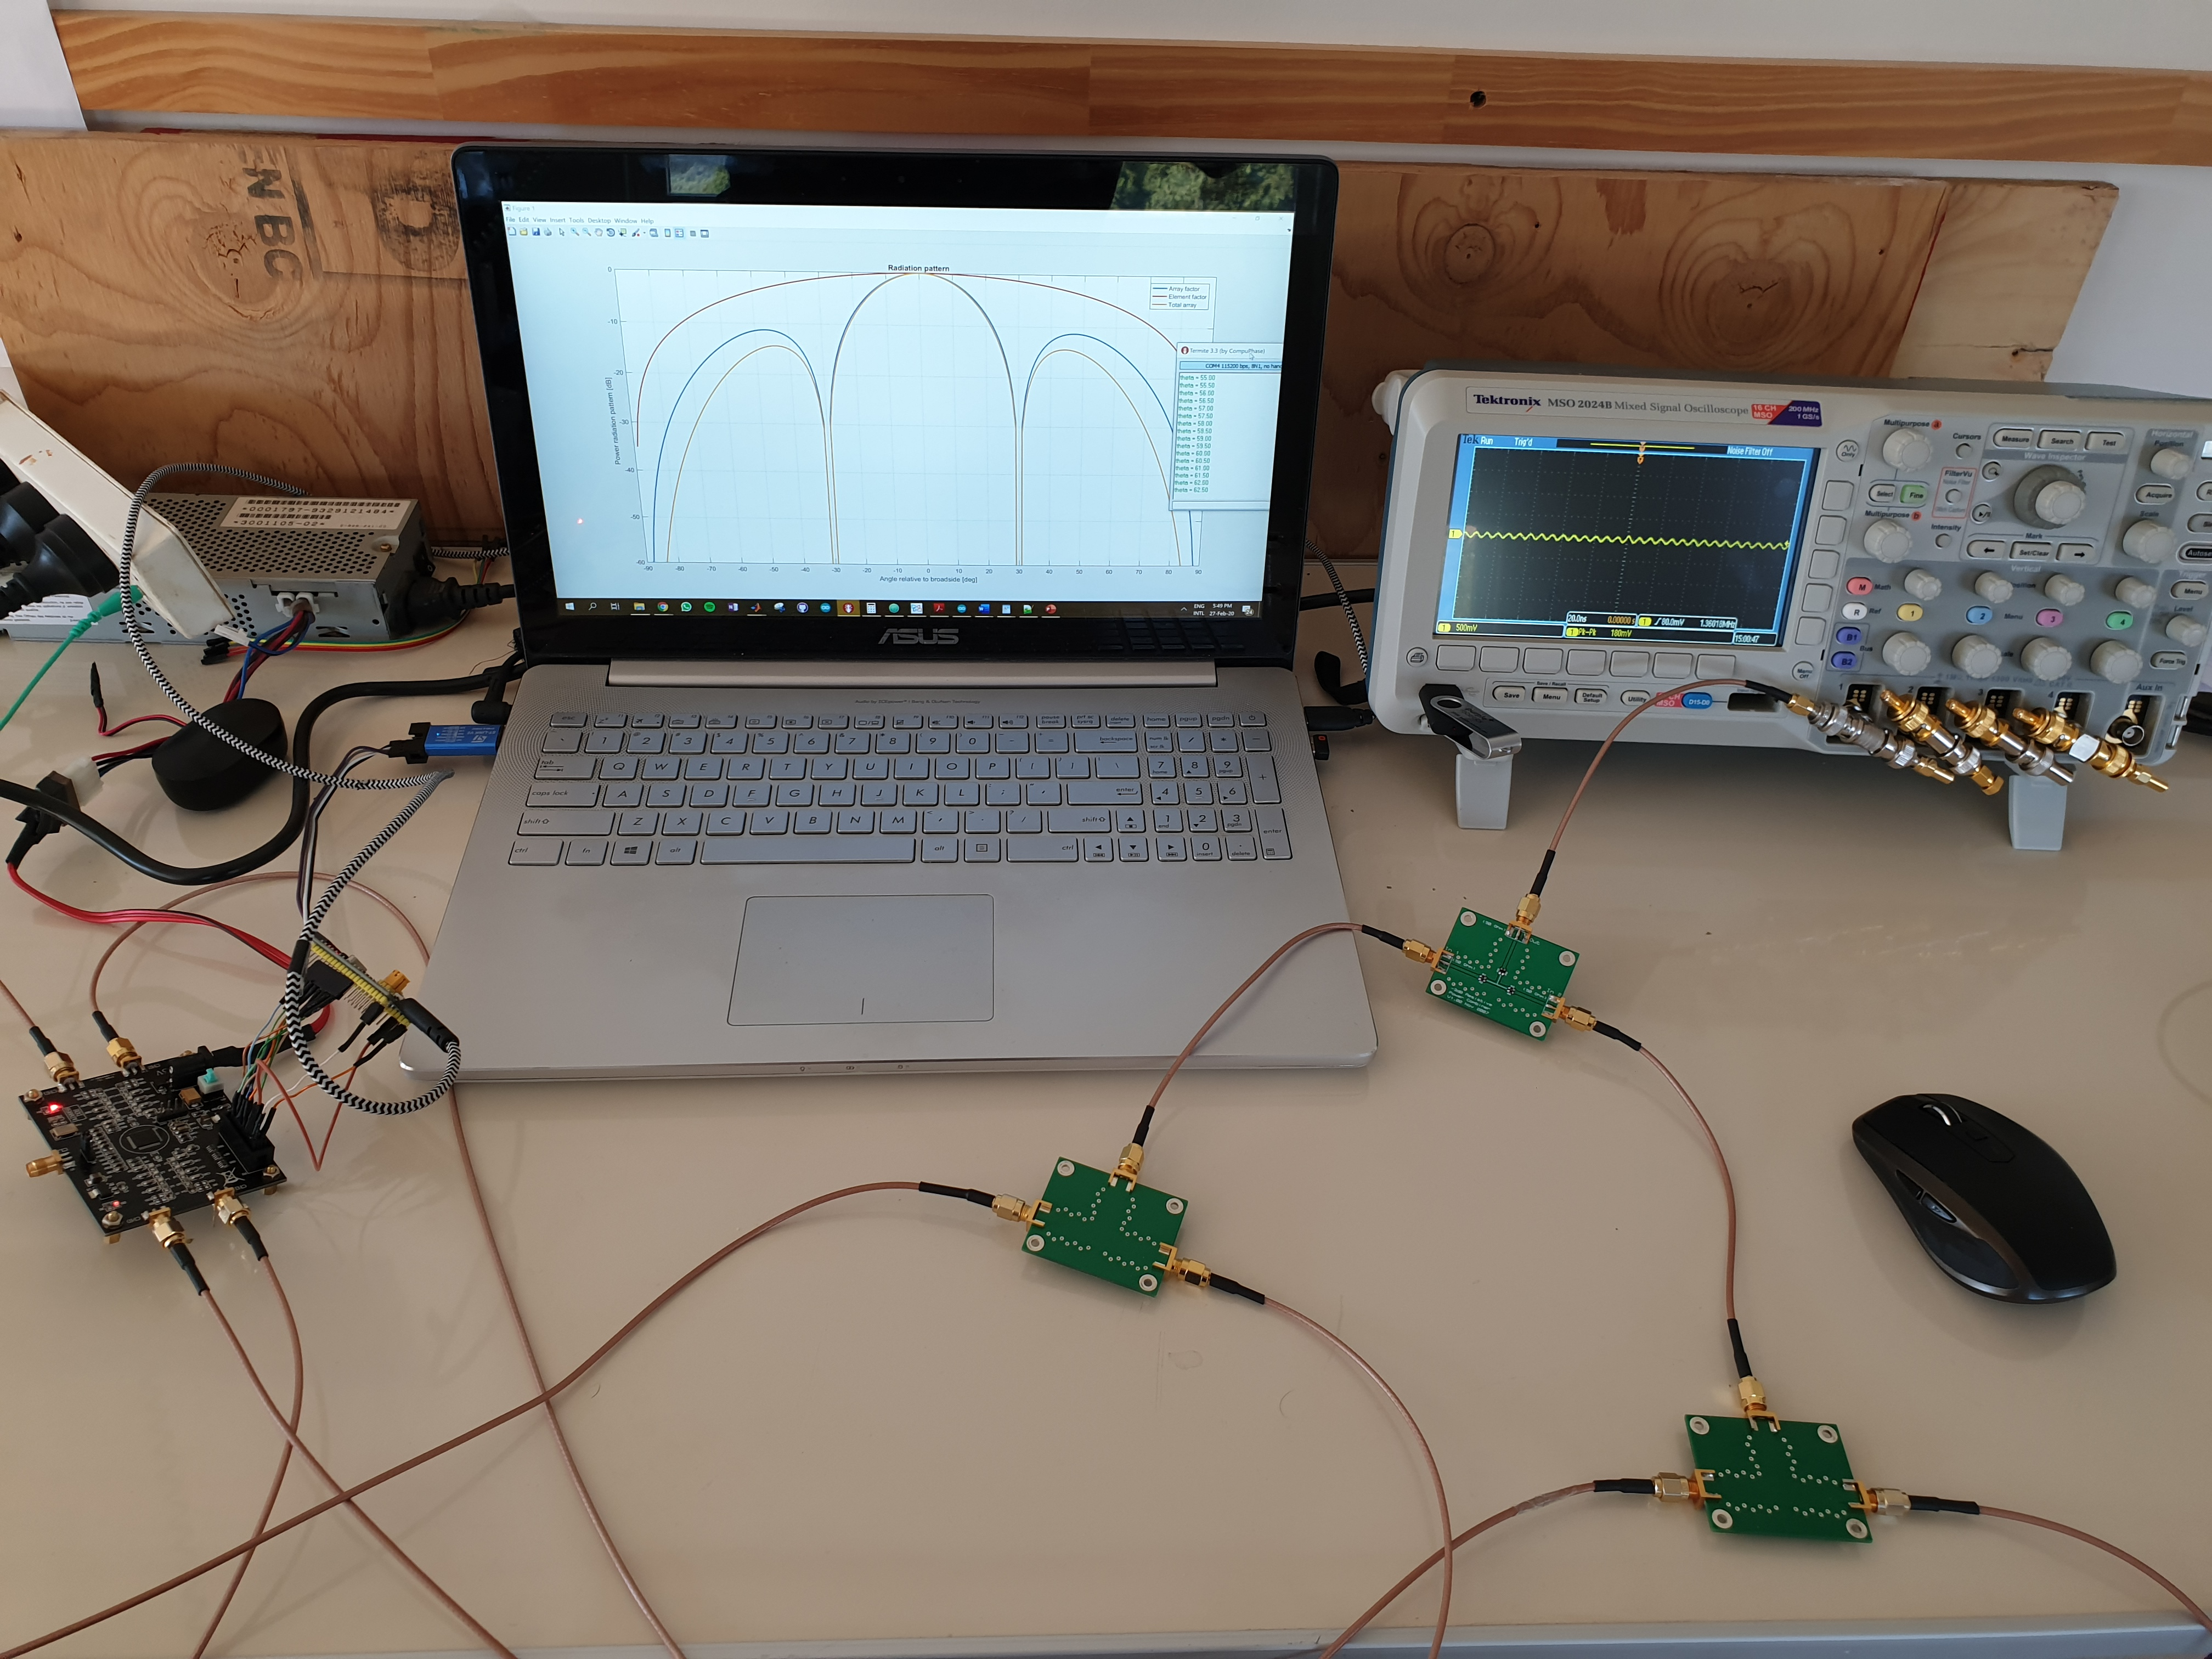
\includegraphics[width=\linewidth/2]{../images/setup-apuntamiento-1.jpg}&
      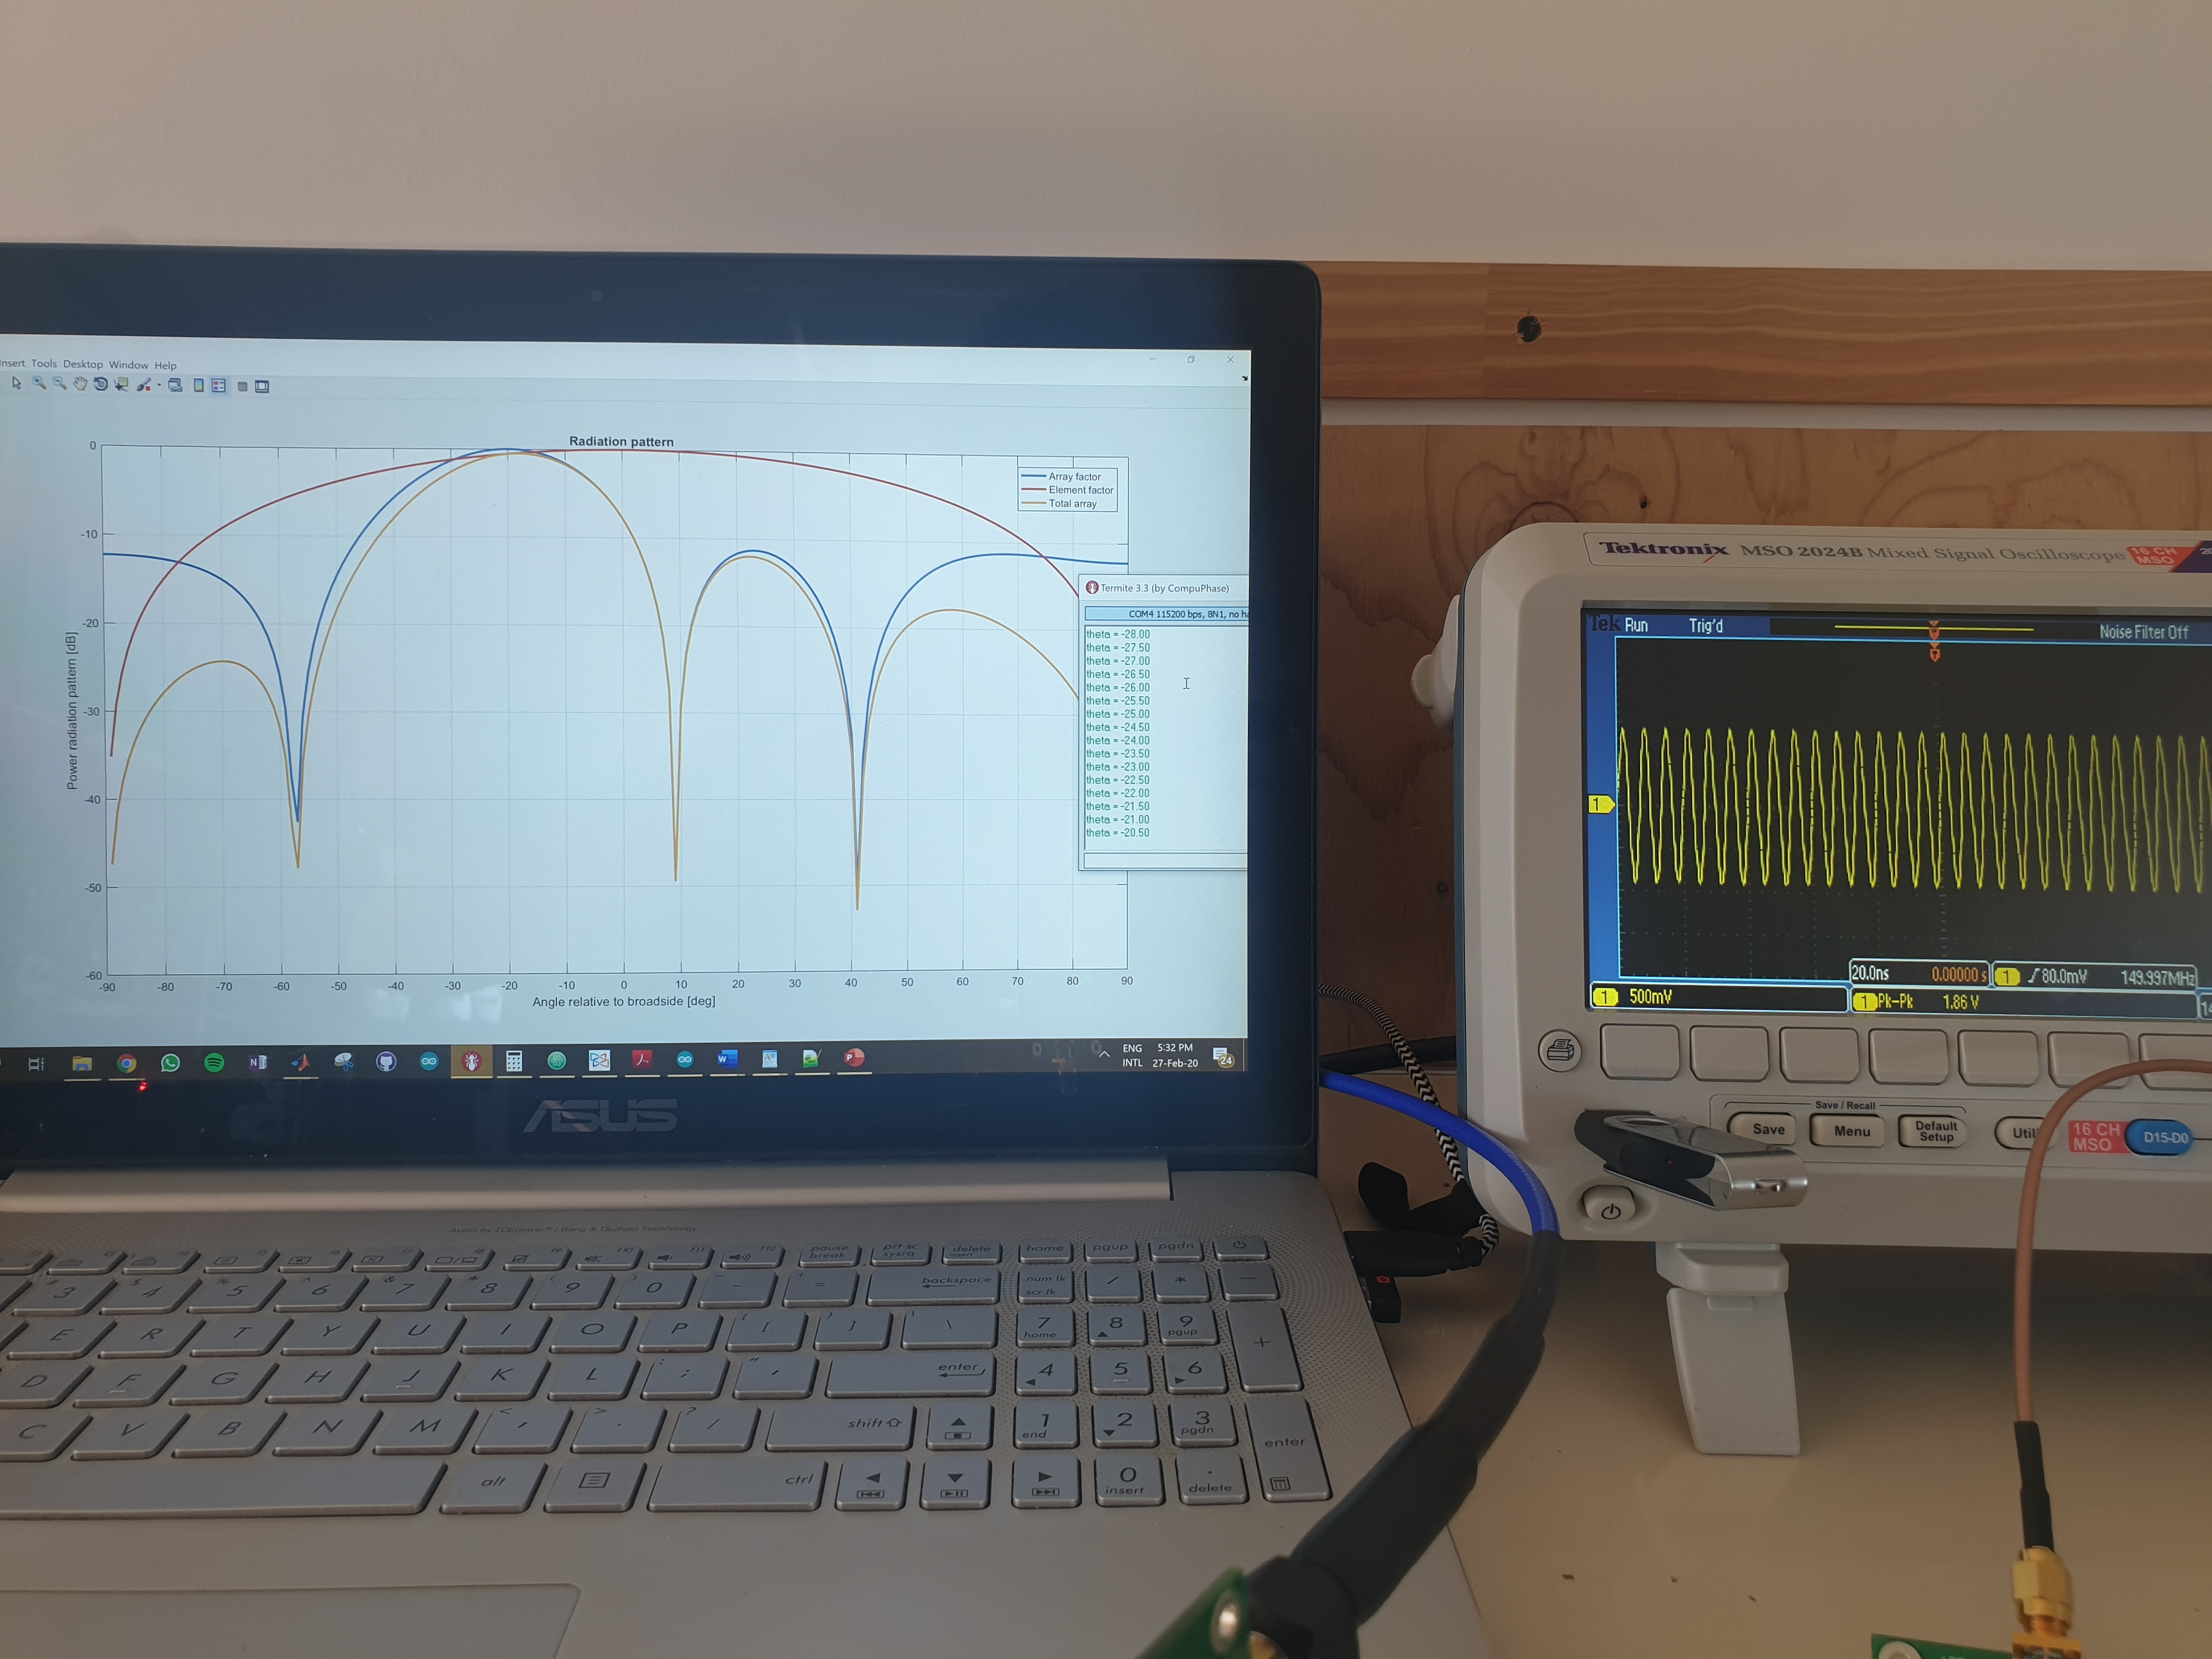
\includegraphics[width=\linewidth/2]{../images/setup-apuntamiento-2.jpg}\\
    \end{tabular}

    \caption{Configuración usada para la verificación del apuntamiento de haz.}
    \label{fig:setup-apuntamiento}
  \end{figure}

\end{standalone}
\end{document}
